\documentclass[12pt]{article}
\usepackage[utf8]{inputenc}
\usepackage{graphicx}
\usepackage{amsmath}
\usepackage{geometry}
\usepackage{booktabs}
\usepackage{float}
\usepackage{subcaption}
\geometry{a4paper, margin=1in}

\begin{document}

\begin{titlepage}
    \centering

    % University logo
    
\includegraphics[width=0.45\textwidth]{images/ozu_logo.png}\\[3cm]

    % Course
    {\large \textbf{EE 350 -- Electronics II}}\\[1cm]

    % Semester
    {\large \textbf{Spring 2025/26}}\\[1cm]

    % Lab number
    {\large \textbf{PRELAB 4}}\\[1cm]

    % Lab title
    {\large \textbf{Succesive Approximation Register}}\\[5cm]

    % Submission info
    \begin{center}
        {\normalsize \textbf{Submitted by:} Ömer Faruk AVCI}\\[0.4cm]
        {\normalsize \textbf{Student ID:} S034113}\\[0.4cm]
        {\normalsize \textbf{Date of Submission:} 22.04.2026} 
    \end{center}

\end{titlepage}


\newpage

\section*{Objective}
In this pre-lab, we implement a Successive Approximation Register (SAR) Analog-to-Digital Converter (ADC) using the Proteus Design Suite. The goal is to study the interaction between digital control logic and analog signal conditioning. An Arduino Uno serves as the controller, generating a PWM signal that is converted to DC via an RC Low-Pass Filter. This voltage is compared against an unknown reference $V_{ref}$ using an Op-amp comparator to drive the bit-by-bit decision logic.

\section*{SAR ADC Implementation with Proteus}

The circuit was constructed in Proteus using the Arduino drivers and a Virtual Terminal for serial monitoring. The design uses an RC Low-Pass Filter ($R = 47\,k\Omega$, $C = 10\,\mu F$) to smooth the PWM output from Pin 9. This DC level is fed into the analog comparator against the input $V_{ref}$.

\begin{figure}[H]
    \centering
    
\includegraphics[width=0.7\textwidth]{images/circuit.png}
    \caption{Proteus Schematic}
    \label{fig:circuit}
\end{figure}

The simulation was verified using the provided \texttt{.hex} firmware. The Virtual Terminal displays each trial bit as the algorithm converges.

\subsection*{Simulation Results}

\begin{figure}[H]
     \centering
     \begin{subfigure}[b]{0.31\textwidth}
         \centering
         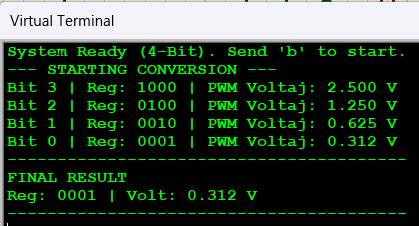
\includegraphics[width=\textwidth]{images/4bit_1v.png}
         \caption{4bit 1V}
     \end{subfigure}
     \hfill
     \begin{subfigure}[b]{0.31\textwidth}
         \centering
         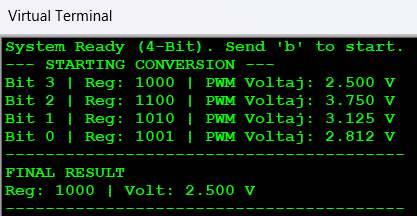
\includegraphics[width=\textwidth]{images/4bit_2_5v.png}
         \caption{4bit 2.5V}
     \end{subfigure}
     \hfill
     \begin{subfigure}[b]{0.31\textwidth}
         \centering
         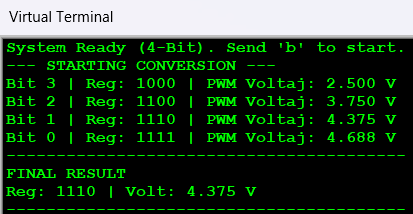
\includegraphics[width=\textwidth]{images/4bit_4v.png}
         \caption{4bit 4V}
     \end{subfigure}
     
     \vspace{10pt}

     \begin{subfigure}[b]{0.31\textwidth}
         \centering
         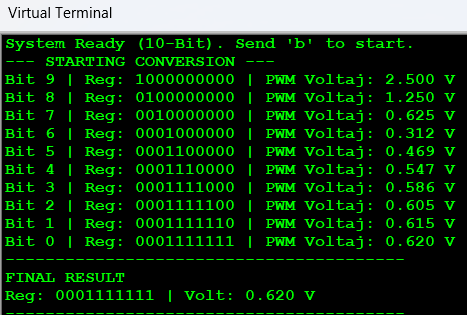
\includegraphics[width=\textwidth]{images/10bit_1v.png}
         \caption{10bit 1V}
     \end{subfigure}
     \hfill
     \begin{subfigure}[b]{0.31\textwidth}
         \centering
         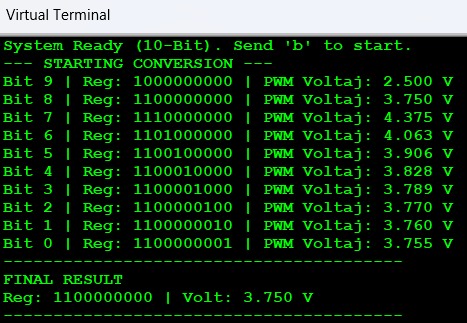
\includegraphics[width=\textwidth]{images/10bit_2_5v.png}
         \caption{10bit 2.5V}
     \end{subfigure}
     \hfill
     \begin{subfigure}[b]{0.31\textwidth}
         \centering
         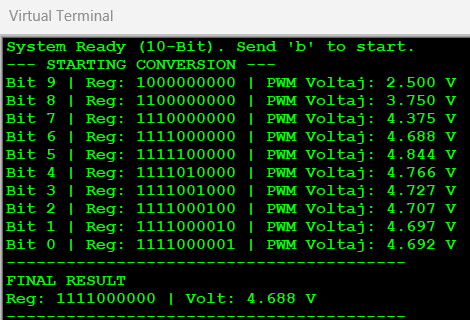
\includegraphics[width=\textwidth]{images/10bit_4v.png}
         \caption{10bit 4V}
     \end{subfigure}
        \caption{Virtual Terminal outputs for different resolutions and input voltages.}
        \label{fig:results_grid}
\end{figure}

\begin{table}[H]
    \centering
    \begin{tabular}{cccc}
        \toprule
        \textbf{Input $V_{ref}$} & \textbf{Final Code (4-bit)} & \textbf{Final Code (10-bit)} & \textbf{Measured (4-bit)} \\ \midrule
        1.0\,V & \texttt{0011} & \texttt{0001111111} & 0.312\,V \\
        2.5\,V & \texttt{1000} & \texttt{1100000000} & 2.500\,V \\
        4.0\,V & \texttt{1110} & \texttt{1111000000} & 4.375\,V \\ \bottomrule
    \end{tabular}
    \caption{Summary of Simulation Measurements}
\end{table}

\section*{Theoretical Calculation}

The quantization step size $Q$ and maximum error $\epsilon_{max}$ for $V_{FS} = 5V$:
\begin{itemize}
    \item \textbf{4-Bit ADC:} $Q = 5/16 = 0.3125\,V$. $\epsilon_{max} = \pm 0.1563\,V$.
    \item \textbf{10-Bit ADC:} $Q = 5/1024 \approx 4.88\,mV$. $\epsilon_{max} \approx \pm 2.44\,mV$.
\end{itemize}

\begin{table}[H]
    \centering
    \begin{tabular}{|c|c|c|c|c|}
        \hline
        & \multicolumn{2}{c|}{\textbf{4-Bit ADC}} & \multicolumn{2}{c|}{\textbf{10-Bit ADC}} \\ \hline
        \textbf{Input $V_{ref}$} & $Q$ (V) & $\epsilon_{max}$ (V) & $Q$ (V) & $\epsilon_{max}$ (V) \\ \hline
        1.0\,V & 0.3125 & $\pm$0.1563 & 0.00488 & $\pm$0.00244 \\ \hline
        2.5\,V & 0.3125 & $\pm$0.1563 & 0.00488 & $\pm$0.00244 \\ \hline
        4.0\,V & 0.3125 & $\pm$0.1563 & 0.00488 & $\pm$0.00244 \\ \hline
    \end{tabular}
    \caption{Theoretical Quantization Values}
\end{table}

\section*{Explanation and Reflection}

The circuit approximates the input voltage through a binary search. Starting from the MSB, the Arduino sets a bit, checks the comparator output, and keeps the bit only if the filtered PWM voltage is below $V_{ref}$. 

In the 4-bit simulation, results stay within the theoretical $\pm 0.156V$ range. However, the 10-bit results show significant errors. This is caused by the RC filter's time constant ($\tau = 0.47\,s$). The 100\,ms firmware delay is too short for the capacitor to settle at 10-bit precision. To fix this, we would need to increase the delay or use a smaller $R$ or $C$.

\end{document}